\documentclass[border=6pt]{standalone}
\usepackage{tikz}
\usetikzlibrary{arrows.meta,positioning,calc}
\begin{document}
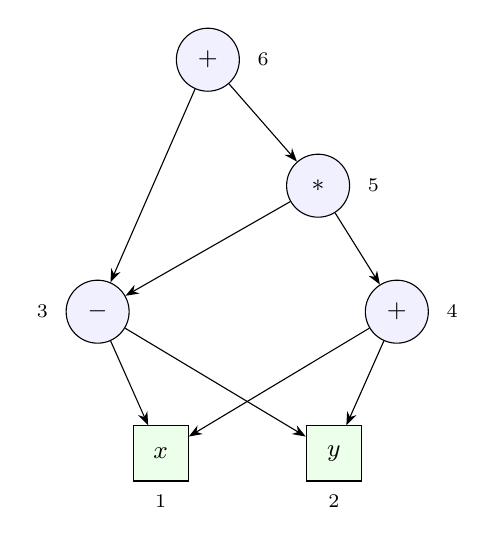
\begin{tikzpicture}[>=Stealth,font=\small,
 op/.style={draw,circle,minimum size=0.8cm,inner sep=0pt,fill=blue!6},
 lf/.style={draw,rectangle,minimum size=0.7cm,inner sep=0pt,fill=green!8}]
\node[op] (n6) at (2,5.4) {$+$}; \node[right=0.1cm of n6,font=\scriptsize] {6};
\node[op] (n5) at (3.4,3.8) {$*$}; \node[right=0.1cm of n5,font=\scriptsize] {5};
\node[op] (n3) at (0.6,2.2) {$-$}; \node[left=0.1cm of n3,font=\scriptsize] {3};
\node[op] (n4) at (4.4,2.2) {$+$}; \node[right=0.1cm of n4,font=\scriptsize] {4};
\node[lf] (x) at (1.4,0.4) {$x$}; \node[below=0.05cm of x,font=\scriptsize] {1};
\node[lf] (y) at (3.6,0.4) {$y$}; \node[below=0.05cm of y,font=\scriptsize] {2};
\draw[->] (n6) -- (n3);
\draw[->] (n6) -- (n5);
\draw[->] (n5) -- (n3);
\draw[->] (n5) -- (n4);
\draw[->] (n3) -- (x);
\draw[->] (n3) -- (y);
\draw[->] (n4) -- (x);
\draw[->] (n4) -- (y);
\end{tikzpicture}
\end{document}
